\documentclass[paper=a4, fontsize=11pt]{scrartcl} % A4 paper and 11pt font size

%----------------------------------------------------------------------------------------
%	PACKAGES
%----------------------------------------------------------------------------------------
\usepackage[T1]{fontenc} % Use 8-bit encoding that has 256 glyphs
\usepackage{fourier} % Use the Adobe Utopia font for the document - comment this line to return to the LaTeX default
\usepackage[english]{babel} % English language/hyphenation
\usepackage{amsmath,amsfonts,amsthm} % Math packages
\usepackage{sectsty} % Allows customizing section commands
\usepackage{fancyhdr} % Custom headers and footers
\usepackage{tabularx, outlines, framed, varwidth, enumitem, graphicx, listings, color, qtree, float, subcaption, newfloat}
\usepackage[left=0.5in, right=0.5in, top=3in, bottom=.25in]{geometry}
\geometry{}

%----------------------------------------------------------------------------------------
%	SET CUSTOMIZATIONS AND FUNCTIONS
%----------------------------------------------------------------------------------------
\sectionfont{\centering \normalfont\scshape} % Make all sections centered, the default font and small caps
\pagestyle{fancyplain} % Makes all pages in the document conform to the custom headers and footers
\fancyhead{} % No page header - if you want one, create it in the same way as the footers below
\fancyfoot[L]{} % Empty left footer
\fancyfoot[C]{} % Empty center footer
\fancyfoot[R]{\thepage} % Page numbering for right footer
\renewcommand{\headrulewidth}{0pt} % Remove header underlines
\renewcommand{\footrulewidth}{0pt} % Remove footer underlines
\setlength{\headheight}{0pt} % Customize the height of the header

\DeclareFloatingEnvironment[fileext=lod]{diagram}

\numberwithin{equation}{section} % Number equations within sections (i.e. 1.1, 1.2, 2.1, 2.2 instead of 1, 2, 3, 4)
\numberwithin{figure}{section} % Number figures within sections (i.e. 1.1, 1.2, 2.1, 2.2 instead of 1, 2, 3, 4)
\numberwithin{table}{section} % Number tables within sections (i.e. 1.1, 1.2, 2.1, 2.2 instead of 1, 2, 3, 4)

\graphicspath{{./figures/}}
%\setlength\parindent{0pt} % Removes all indentation from paragraphs - comment this line for an assignment with lots of text

\makeatletter
	\newcommand*\variableheghtrulefill[1][.4\p@]
	{%
		\leavevmode
		\leaders \hrule \@height #1\relax \hfill
		\null
	}
\makeatother

\lstset
{
	language=C++,
%	basicstyle=\ttfamily,
%	keywordstyle=\color{blue}\ttfamily,
%	stringstyle=\color{red}\ttfamily,
%	commentstyle=\color{green}\ttfamily,
%	morecomment=[l][\color{magenta}]{\#}
	keywordstyle=\color{blue},
	stringstyle=\color{red},
	commentstyle=\color{green},
	morecomment=[l][\color{magenta}]{\#}
}

%----------------------------------------------------------------------------------------
%	USEFUL COMMANDS
%----------------------------------------------------------------------------------------
%	\makebox[\textwidth][c]{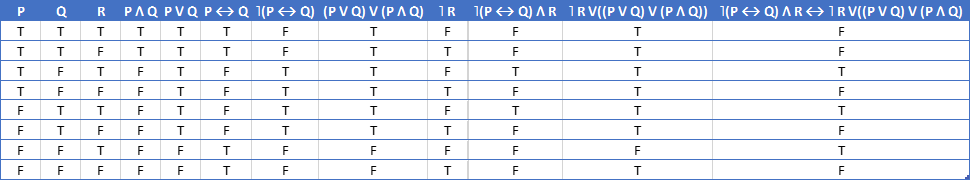
\includegraphics[width=.9\pagewidth]{p2-table}}

%	\newgeometry{top=.75in, bottom=.75in, left=.25in,right=.25in}
%	\newgeometry{top=.75in, bottom=.75in, left=1.25in,right=1.25in}

%	\lstinputlisting[firstline=4]{CMPSC360_Homework.cpp}

%\Tree
%	[.<root> [.<left> ][.<middle> ][.<right> ]]

%----------------------------------------------------------------------------------------
%	TITLE SECTION
%----------------------------------------------------------------------------------------

\newcommand{\horrule}[1]{\rule{\linewidth}{#1}} % Create horizontal rule command with 1 argument of height
% \title{Template: Homework 1}
\title{	
\normalfont \normalsize 
%\textsc{Rutgers University, Real Analysis I} \\ [25pt] % Your university, school and/or department name(s)
\horrule{0.5pt} \\[0.4cm] % Thin top horizontal rule
\huge STAT 463: Homework 10 \\ % The assignment title
\horrule{2pt} \\[0.5cm] % Thick bottom horizontal rule
}

\author{\textbf{\underline{Name:}}Kyle Salitrik | \textit{\textbf{\underline{ID\#:}} 997543474} | \textit{\textbf{\underline{PSU ID:}} kps168}} % Your name

\date{\normalsize\today} % Today's date or a custom date

\begin{document}

\maketitle % Print the title
\newgeometry{top=.75in, bottom=.75in, left=1.25in,right=1.25in}

%----------------------------------------------------------------------------------------
%	PROBLEM 1
%----------------------------------------------------------------------------------------



\section*{\variableheghtrulefill[.25ex]\quad Problem 1 \quad\variableheghtrulefill[.25ex]}
\subsection*{a)}
Based on the time series and both the ACF and PACF plots, it appears that the entire time series is random noise.

\makebox[\textwidth][c]{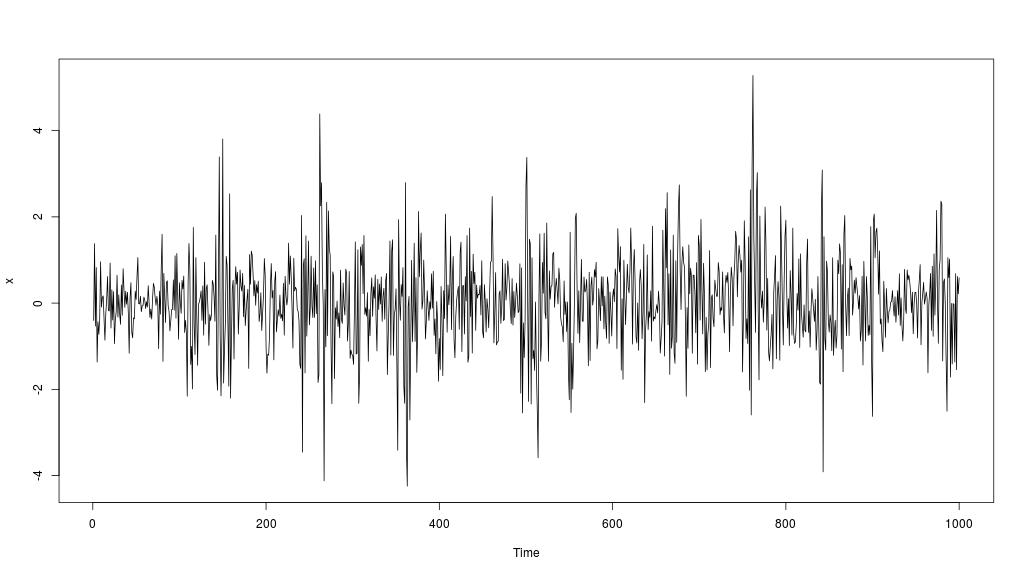
\includegraphics[scale=.5]{p1_a_1.png}}
\makebox[\textwidth][c]{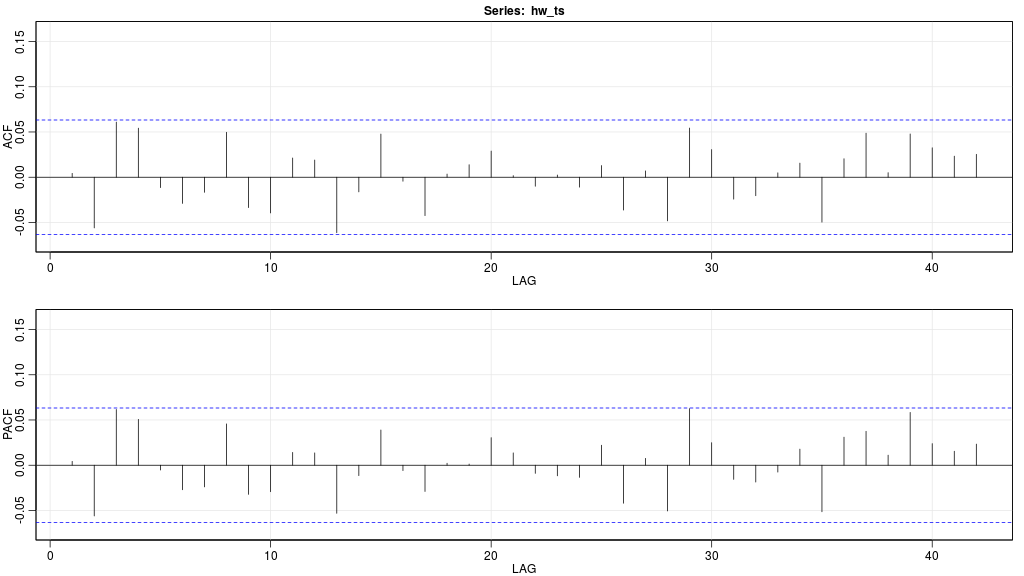
\includegraphics[scale=.5]{p1_a_2.png}}

\subsection*{b)}
Using the squared series values, the ACF and PACF Possibly suggest an AR(1) or ARMA(1,1).
\makebox[\textwidth][c]{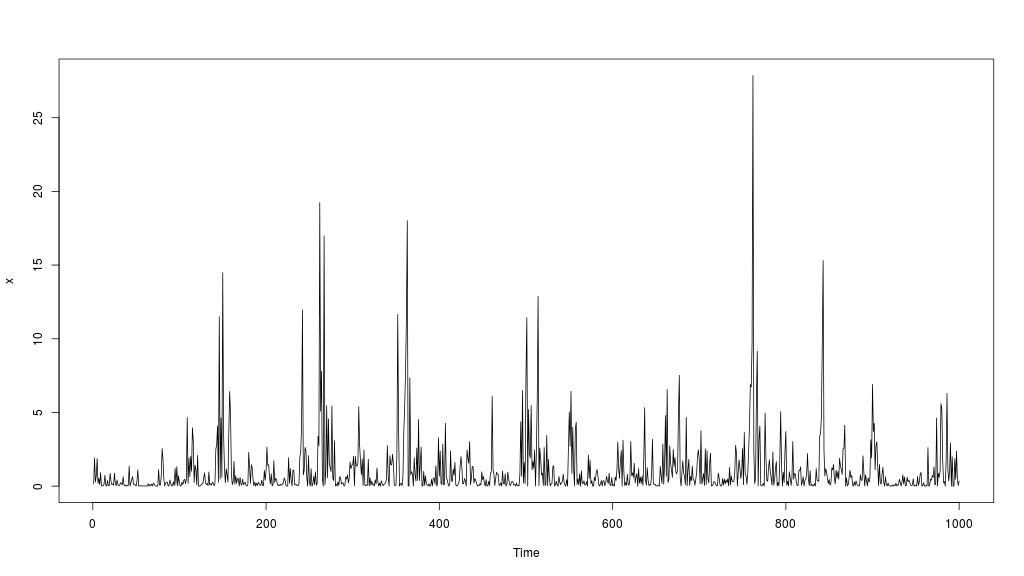
\includegraphics[scale=.5]{p1_b_1.png}}
\makebox[\textwidth][c]{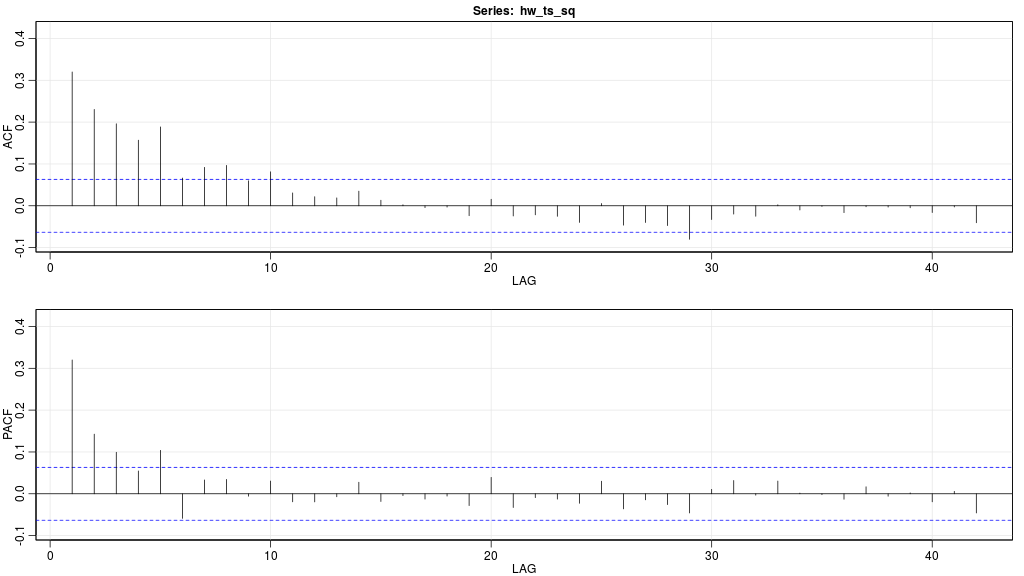
\includegraphics[scale=.5]{p1_b_2.png}}

\subsection*{c)}
Based on the ARCH and GARCH models, the GARCH had a lower AIC, BIC, SIC, and HQIC. Normality tests show that the residuals have a normal distribution
\lstinputlisting[language=]{listings/garch_stats.txt}

\subsection*{d)}
\begin{flalign*}
	&y = \sigma_{t}\epsilon_{t} &\\
	&\sigma_{t} = sqrt{0.09622 + 0.31894y^2_{t-1} + 0.60802\sigma^2_{t-1}} &\\
	&\epsilon \overset{iid}{\sim} N(0,1) &
\end{flalign*}

\subsection*{e)}
\lstinputlisting[language=]{listings/garch_predict.txt}

\section*{\variableheghtrulefill[.25ex]\quad Problem 2 \quad\variableheghtrulefill[.25ex]}

\subsection*{a)}
Looking at the 'none', 'both', 'trend', and 'constant' models, the 'none' produced the highest adjusted $R^2$ values for all models. These are the resulting models:

\begin{flalign*}
	&\hat{B}_{t} = 1.05330 B_{t-1} - 0.30720 M_{t-1} + 0.24882 K_{t-1} &\\
	&\hat{M}_{t} = 0.14485 B_{t-1} + 0.56676 M_{t-1} + 0.27974 K_{t-1} &\\
	&\hat{K}_{t} = 0.2423 B_{t-1} - 0.4384 M_{t-1} + 1.1886 K_{t-1} &
\end{flalign*}

\subsection*{b)}
Again, for the VAR(2) models, including neither the intercept or constant produced the best model based on adjusted $R^2$ value.
\begin{flalign*}
	&\hat{K}_{t} = -0.09426 t - 0.19763 B_{t-1} + 0.59703 M_{t-1} + 0.81700 K_{t-1} + 1.13432 B_{t-2} - 1.67339 M_{t-2} + 0.33416 K_{t-2} &
\end{flalign*}

\subsection*{c)}
The BIC values are as follows:
\begin{itemize}
	\item BIC1: 8.417481
	\item BIC2: 8.492818
\end{itemize}

Based on these values the BIC for the VAR(1) model indicates that it is the better option.

\subsection*{d)}
Based on the ACF of the residuals for the 3 cities, all values are within the lines of significance.
\makebox[\textwidth][c]{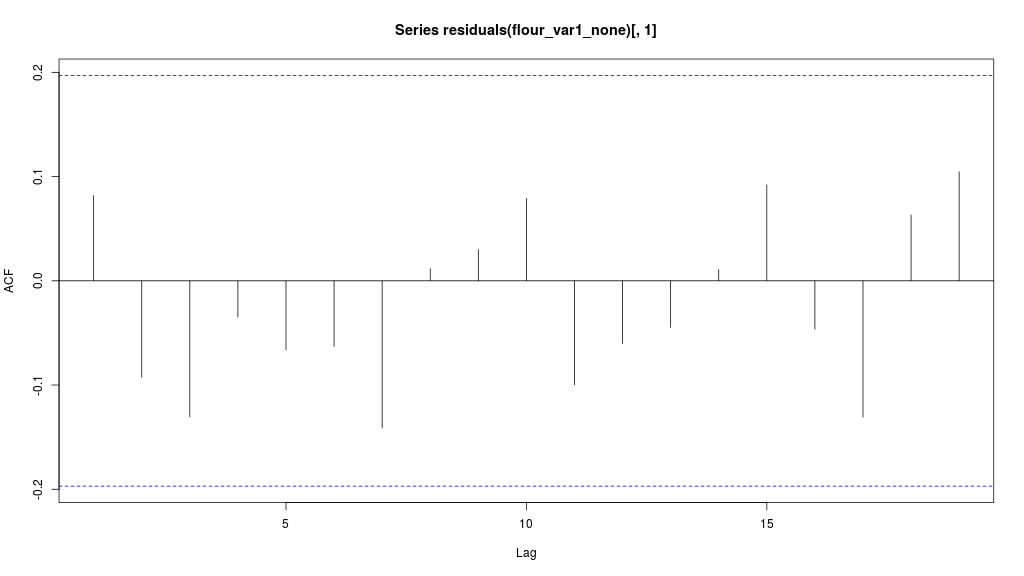
\includegraphics[scale=.5]{p2_d_1.png}}
\makebox[\textwidth][c]{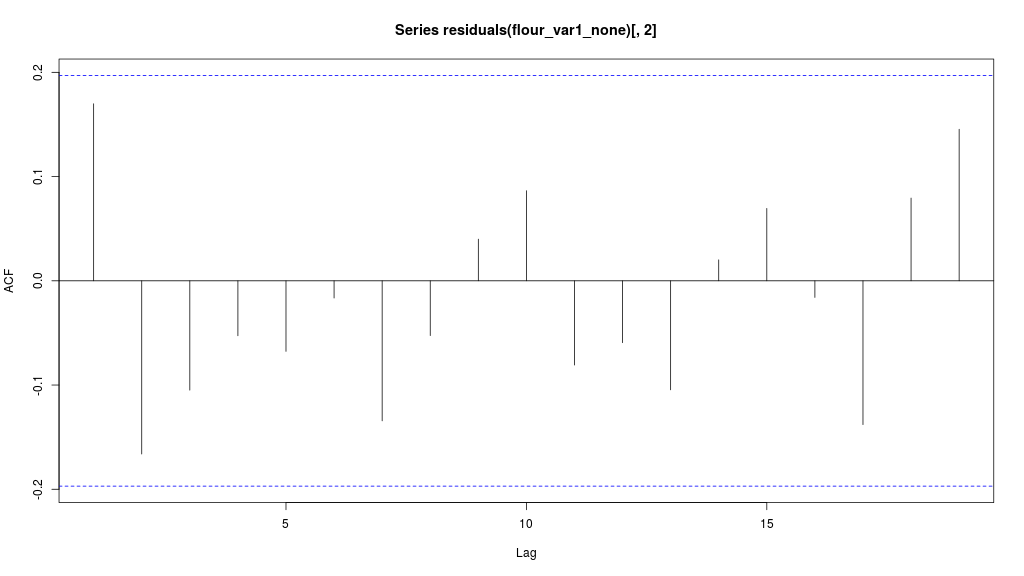
\includegraphics[scale=.5]{p2_d_2.png}}
\makebox[\textwidth][c]{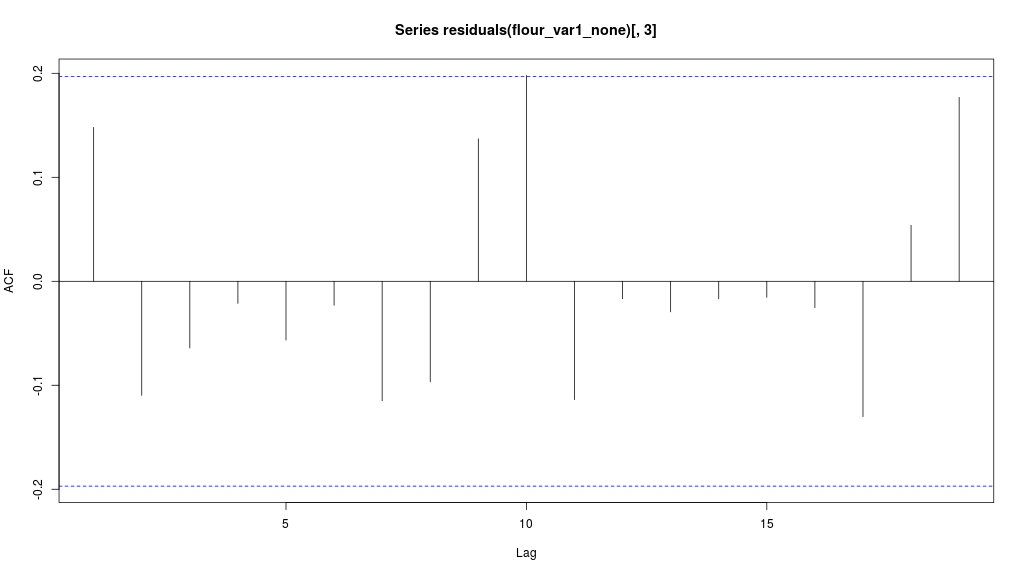
\includegraphics[scale=.5]{p2_d_3.png}}
\end{document}